\documentclass{standalone}
\usepackage[utf8]{vietnam}
\usepackage{amsmath,amsxtra,amssymb,latexsym, amscd,amsthm}
\usepackage{mathptmx} 
\usepackage{mathrsfs}
\usepackage{tikz}
\usetikzlibrary{mindmap,trees,shadows,chains,scopes,shapes.geometric,calc,fadings,intersections}
\def\colorLeft{green!50!yellow!70!red!30!blue}
\def\colorRight{orange}
\def\colorTop{red!80!blue!80}
\begin{document}
	\pagestyle{empty}
	
	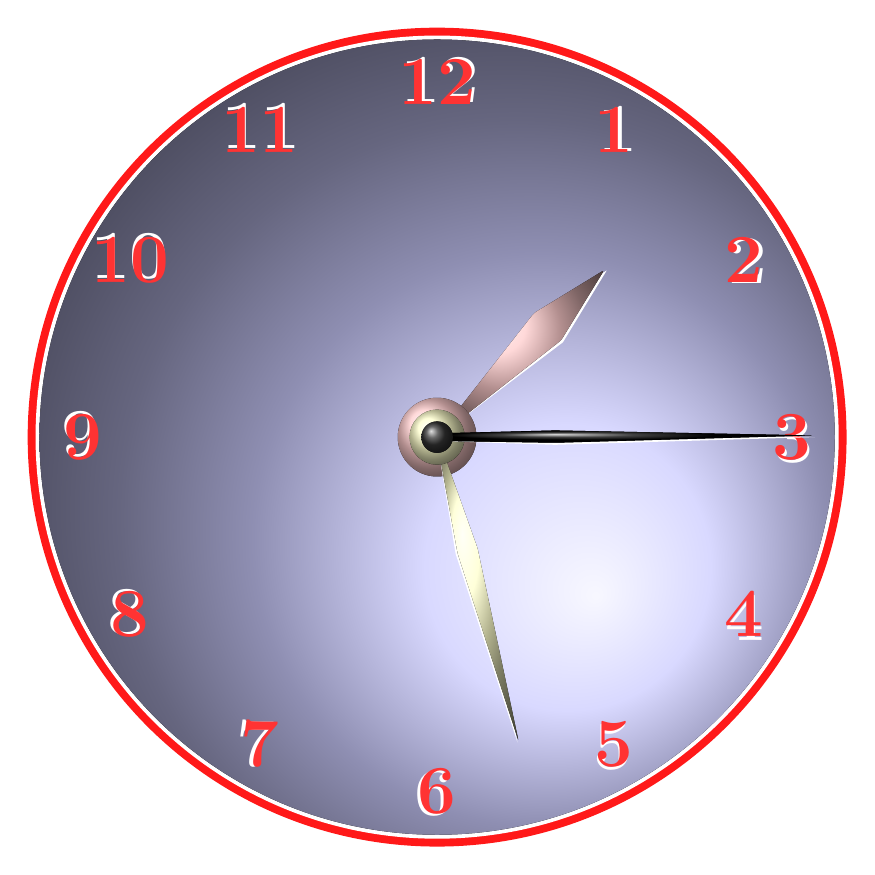
\begin{tikzpicture}[>=stealth]
		\fill [color=red!90] (0,0) circle (5.2);
		\fill [color=white] (0,0) circle (5.1);
		\fill [ball color=blue!20,shading angle={180}] (0,0) circle (5.05);
		
		\foreach \goc/\gio in {60/1,30/2,0/3,-30/4,-60/5,-90/6,-120/7,-150/8,-180/9,-210/10,-240/11,-270/12}{
			\pgfmathsetmacro{\bong}{\goc -0.5}
			\draw[color=white] (\bong:4.53) node {\bf \Huge \gio};
			\draw [color=red!80] (\goc : 4.5) node {\bf\Huge \gio};
		}
		
		\pgfmathsetmacro{\kgio}{45}
		\fill [color = white,opacity=1]
		(\kgio-10: 0.1) -- (\kgio-8:2) -- (\kgio-0.5:3.02) -- (\kgio+6:2) -- (\kgio+8:0.1);
		\fill [ball color =red!20,rounded corners=1,opacity=1]
		(\kgio-9: 0.1) -- (\kgio-7:2) -- (\kgio:3) -- (\kgio+7:2) -- (\kgio+9:0.1);
		\fill [ball color=red!20] (0,0) circle (0.5);
		
		\pgfmathsetmacro{\kphut}{-75}
		\fill [color = white,opacity=1]
		(\kphut-11: 0.1) -- (\kphut-6:1.5) -- (\kphut-0.25:4.01) -- (\kphut+4:1.5) -- (\kphut+9:0.1);
		\fill [ball color =yellow!20,  rounded corners=1,opacity=1]
		(\kphut-10: 0.1) -- (\kphut-5:1.5) -- (\kphut:4) -- (\kphut+5:1.5) -- (\kphut+10:0.1);
		\fill [ball color=yellow!20] (0,0) circle (0.35);
		
		\pgfmathsetmacro{\kgiay}{rand}
		\fill [color = white,opacity=1]
		(\kgiay-31: 0.1) -- (\kgiay-4:1.5) -- (\kgiay-0.25:4.8) -- (\kgiay+2:1.5) -- (\kgiay+29:0.1);
		\fill [ball color =black, rounded corners=1,opacity=1]
		(\kgiay-30: 0.1) -- (\kgiay-3:1.5) -- (\kgiay:4.78) -- (\kgiay+3:1.5) -- (\kgiay+30:0.1);
		\fill [ball color=black!80] (0,0) circle (0.2);
		
	\end{tikzpicture}
\end{document}